\documentclass[11pt]{article}
\usepackage[T1]{fontenc}
\usepackage[utf8]{inputenc}
\usepackage{xcolor}
\definecolor{darkblue}{rgb}{0,0,0.5}
\usepackage[colorlinks=true,allcolors=darkblue]{hyperref}
\usepackage{amsmath}
\usepackage{amssymb}
\usepackage{booktabs}
\usepackage{multirow}
\usepackage{enumitem}
\usepackage{multirow}
\setlist{noitemsep}
\usepackage{caption}
\usepackage{subcaption}
\usepackage{graphicx}
\graphicspath{{image/}}
\usepackage[sorting=ynt,style=authoryear,uniquename=false]{biblatex}
\addbibresource{paper.bib}

\title{Variational autoencoders for argumentation representation learning}
\author{%
  Kuan Yu, Jan Milde\\
  \texttt{\{kuanyu, jmilde\}@uni-potsdam.de}\\
  Master's Program in \emph{Cognitive Systems}\\
  University of Potsdam}
\date{March 2019}

\begin{document}
\maketitle

\begin{abstract}
  We trained two recurrent variational autoencoders for learning argumentation representation
  with datasets assembled from the internet,
  one for sentence embedding and another for post embedding.
  We evaluated the learned representation in supervised tasks
  with a third dataset containing online debate posts annotated with labels
  regarding the content of argumentation.
  The results were a mixture of successes and failures.
  This paper gives a detailed analysis.
\end{abstract}

\section{Introduction}\label{sec:introduction}

Argumentation mining is a developing field of natural language processing
in pursuit of the automatic identification and extraction of information from argumentative texts.
We are particularly interested in the content of argumentation,
such as the topic of debate and the argumentative reason.
This project explored the unsupervised learning of argumentation representation with variational autoencoders,
and applied the learned representation in supervised tasks for evaluation.
The results fell short of our expectations,
but our explorations were fruitful and educational.
The implementation for our experiments is openly available.%
\footnote{\url{https://github.com/argsim/argsim}}

We start this paper with a description of the theoretical and technical background
(Section~\ref{sec:background}).
Then we explain the general setup of our experiments and detail the training of our unsupervised models
(Section~\ref{sec:experiments}).
Next we present and examine the results of supervised evaluation
(Section~\ref{sec:results}).
At last we conclude our paper with a summary and some discussions (Section~\ref{sec:conclusion}).

\section{Background}\label{sec:background}

\subsection{Argumentation embedding}\label{sec:argum-simil}

There is an abundance of data available for argumentation mining from discussions led online which,
if being ordered and structured, could give a well rounded view on a topic.
However, data labeling is time consuming and labor intensive.
Effective unsupervised methods for argumentation mining are desired.
\textcite{boltuvzic2015identifying} experimented with unsupervised clustering of argumentative sentences based on the similarity of their sentence embeddings,
which were derived by adding up all the word embeddings of the sentence.

Following the invention of the word2vec model \parencite{mikolov2013efficient}, word embeddings have risen to popularity and have become a standard when working with text.
The reason for the success is that the embedding model learns a meaningful representation space.
For example, within this space are linear substructures for gender representation such that the distance between ``man'' and ``woman'' would be highly similar to the distance between ``king'' and ``queen''.
Similarity metrics such as the cosine similarity between word vectors prove to be an effective way to represent their semantic similarity.
In general, the closest neighbors are highly related. I.e.\ conjugations, synonyms, or words of the same topic \parencite{pennington2014glove}.
This motivated researchers to explore methods to embed longer texts, such as sentences or paragraphs.
As one of the first steps in this direction, simply adding up weighted word vectors to be sentence embeddings and weighted sentence embeddings to be paragraph embeddings was a working approach \parencite{arora2016simple}.
It could be shown that sentence or paragraph embeddings can also have a meaningful spacial interpretation \parencite{dai2015document}.
This makes research for sentence or paragraph embeddings highly relevant for the field of argumentation similarity.
However, the composition of texts from words is a process far more complicated than the linear combination of word vectors.
Emergent linguistic properties such as the grammar formalism and the writing style require more sophisticated modeling tools.
Hence as of now, the search for the best text embedding method is still in progress.

\subsection{Recurrent variational autoencoder}\label{sec:recurr-vari-auto}

Probabilistic graphical models based on the principle of Boltzmann machines
saw the success of data-driven modeling \parencite{ackley1985learning}.
In this connectionist approach, a generative model is trained on the raw data.
Such a generative model typically consists of visible and hidden nodes.
The data is input to the visible nodes of the model,
and values for the hidden nodes are computed through probabilistic inference.
A trained model can be used to generate data from a particular configuration of hidden values, namely the hidden state,
and can also be used for inferring the hidden state which explains the structure of a given data point.
The hidden states are constrained by the architecture of the model to have simpler structures than the raw data,
which makes these models useful for extracting non-linear features from the raw data
for linear classification or clustering \parencite{hinton2006reducing}.
Exact inference in a generative model is often intractable,
for which approximation methods such as variational inference is usually used.
An effective training method for deep belief networks triggered the revival of artificial neural networks
in statistical machine learning \parencite{hinton2006fast}.
Modern variants of generative models have maintained their popularity
in the form of differentiable generative networks which allow for effective training through backpropagation,
such as variational autoencoders (VAEs) \parencite{kingma2013auto}.

\begin{figure}
  \centering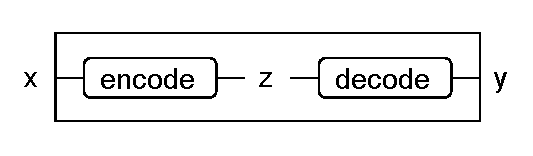
\includegraphics[width=0.7\linewidth]{vae.pdf}
  \caption[]{\label{fig:vae}A variational autoencoder (\(x = y\)).}
\end{figure}

A VAE consists of an encoder and a decoder (Figure~\ref{fig:vae}).
The encoder is a neural network which receives a data point as input and outputs a latent vector \(z\),
from which the decoder network reconstructs the original data point.
Conceptually, the decoder is a directed graphical model from the latent space to the data space
whereas the encoder performs variational inference in the backward direction.
The components of the latent vector \(z\) are assumed to be independent and identically distributed random variables,
typically following a standard isotropic multivariate normal distribution.
This assumption is enforced during training through backpropagation using the reparameterization trick
where random noises are added to the latent variables.
The training objective is to raise the variational lower bound
by minimizing the Kullback–Leibler divergence (KL) between the distributions
of the latent variables and their assumed prior
while maximizing the likelihood of the training data
or equivalently minimizing the reconstruction error.

\begin{align*}
  \mathcal{L} \left( \theta ; x \right)
  &= \mathbb{E}_{q_{\theta} \left( z | x \right)} [ \log p_{\theta} \left( x | z \right)]
    - \mathtt{KL} \left( q_{\theta} \left( z | x \right) \| p \left( z \right) \right)\\
  &\leq \log p\left(x\right)
\end{align*}

The prior imposed on \(z\) by the KL term in the loss function enforces information
to be encoded in a disentangled manner.
The encoder acts as an embedding function from the data space to the latent space,
where each dimension represents a distinctly interpretable feature of the data.
For this reason,
VAEs serve as an interesting bridge between the connectionist approach and the symbolist approach to data modeling,
which is evident in their capability of separating the style and the content of images \parencite{kingma2014semi}.

\begin{figure}
  \centering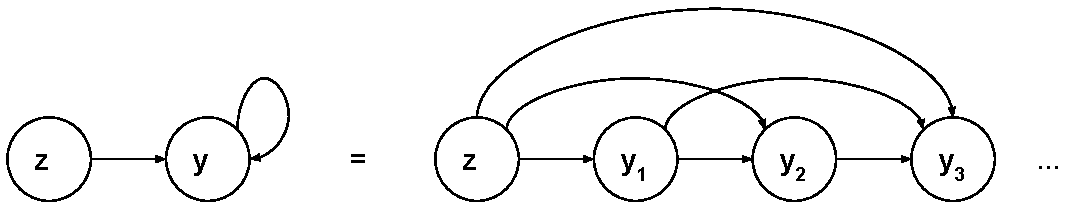
\includegraphics[width=\linewidth]{autoreg.pdf}
  \caption[]{\label{fig:autoreg}An autoregressive decoder models
    the probability of a sequence \(y\) given a latent state \(z\),
    with the sequence factorized causally by position:
    \small{\( p(y \mid z) = p(y_{1} \mid z)\ p(y_{2} \mid y_{1}, z)\ p(y_{3} \mid y_{2}, y_{1}, z)\ \ldots \)}}
\end{figure}

In natural language processing,
VAEs have been successfully applied for
sentence representation learning \parencite{bowman2015generating},
discourse-level diversity learning \parencite{zhao2017learning},
topic model learning \parencite{srivastava2017autoencoding},
semantic space learning \parencite{jang2018recurrent},
and target-level sentiment analysis \parencite{xu2018semi}.

In those applications, recurrent neural networks (RNNs) are a typical choice.
The encoder RNN transforms an input sequence to a single state vector,
while the decoder autoregressively generates an output sequence,
with each step conditioning on the encoded state and previously generated partial sequence (Figure~\ref{fig:autoreg}).
During generation, an output is sampled from the decoder predictions at each step,
and fed back together with the recurrent state for the next step.
Since the search space grows exponentially for such a structure prediction problem,
beam search is commonly used to approximate the optimal solution \parencite{freitag2017beam}.
A cheaper alternative is greedy decoding,
where the sampling is simply performed by picking the prediction with the highest probability.
For training an autoregressive model,
the teacher-forcing method is typically used \parencite{williams1989learning}.
Instead of running the feedback loop,
the true sequence is given as input with a begin-of-sentence symbol padded at the front
to predict the same sequence with an end-of-sentence symbol padded at the end.

\subsection{Sentence piece}\label{sec:sentence-piece}

When treating texts as sequences generated from a set of symbols,
it is common and intuitive to choose words as the symbolic units.
This however has many drawbacks.
The vocabulary size of any corpus is huge, often in an order of magnitude around or above \(10^{6}\),
resulting in a large number of parameters in the input and output layers of the model.
On top of that, due to their power law distribution,
the majority of words in the vocabulary of a language remains unseen in the available training data,
and most words in the observed vocabulary occur infrequently.
Furthermore, morphology is an important part of language,
especially for agglutinative languages,
which can only be modeled at the subword level.
Modeling at the character-level can be effective \parencite{kalchbrenner2016neural}.
However, the sequences become much longer,
making computation prohibitively expensive.
An often adopted compromise is to model a fixed set of frequent words
while segmenting the rest into word pieces using byte-pair encoding (BPE) \parencite{sennrich2015neural}.
An equivalent approach which does not require tokenization is a sentence-piece model \parencite{kudo2018subword}.

Sentence pieces are character ngrams,
which are whole words at the maximum level and single characters at the minimum level.
Segmentation can be performed using BPE or a unigram language model
(with a unigram being a sentence piece).
A sentence-piece model is trained on the data directly based on the frequencies.
A unigram sentence-piece model can be used by picking the optimal segmentation,
or by sampling from the space of all possible segmentations according to the unigram probabilities.

As an example, the phrase ``argumentation mining'' can be segmented in the following ways,
ranked by the sampling likelihood.
(Here \texttt{\_} denotes word boundary and space denotes segmentation.)

\begin{itemize}
  \item \texttt{\_argument ation \_mining}
  \item \texttt{\_argument at ion \_mining}
  \item \texttt{\_argument ation \_ min ing}
  \item \texttt{\_argument ation \_mini ng}
  \item \texttt{\_argument a tion \_mining}
  \item \dots
\end{itemize}

While the sampled segmentations do not always reflect the morphology,
they are often informative and provide potentially unlimited variations from limited data.
Training a model with sentence-piece sampling is an effective regularization technique
and was shown by \textcite{kudo2018subword} to improve the quality of machine translation.

\section{Experiments}\label{sec:experiments}

\subsection{Datasets and preprocessing}\label{sec:datas-prepr}

Three datasets were involved in our experiments,
one for evaluation and two for training.

We trained separate sentence-piece model on each set of training data.
The vocabulary size was set to 8192 with a total character coverage of 99.95\%.
When sentence-piece sampling was applied,
the smoothing parameter was set to \(\alpha = 0.5\) with an unlimited sampling size.

\subsubsection*{Evaluation data}

\begin{table}
  \centering
  \begin{tabular}{lccc}
    \toprule
    Topic & Posts & Sentences (annotated) & Reason labels\\
    \midrule
    Abortion   &~463 &~876 &13\\
    Gay Rights &~560 &~865 &~9\\
    Obama      &~446 &~651 &16\\
    Marijuana  &~432 &~846 &10\\
    \midrule
    Total      &1901 &3238 &48\\
    \bottomrule
  \end{tabular}
  \caption{\label{tab:data-eval}Evaluation data.}
\end{table}

For evaluating the quality of the learned text representation,
we used the stance and reason dataset assembled by \textcite{hasan2014you}.
The dataset consisted of online debate posts on four topics:
\textit{Abortion}, \textit{Gay Rights}, \textit{Obama}, and \textit{Marijuana}.
Each post was annotated with a binary stance in terms of pro and con
and contained an arbitrary number of argumentative sentences annotated with labels for the reason of argumentation
(Table~\ref{tab:data-eval}).
Accompanying the dataset was the partition information of five-fold cross-validation
for stance and reason classification.
This dataset was used in order to have comparable results to \textcite{boltuvzic2015identifying},
but there are several problems within the dataset.
Additional to having duplicate sentences with differed labels and occasional different stances within one post,
the main issue is that often questionable choices are made regarding the labeling (Table~\ref{tab:label-examples}).

\begin{table}
  \centering
  \begin{tabular}{lll}
    \toprule
    Topic & Reason & Sentence\\
    \midrule
    Marijuana & c-health & \multicolumn{1}{p{8cm}}{Smoking a useless plant isn't ``recreational''.} \\
    Marijuana & p-medicine & \multicolumn{1}{p{8cm}}{I’m saying that during jazz’s first creative explosion, weed was a major factor in the community. And yes, lowered stress is an excellent way to make better music.} \\
    GayRights & c-born & \multicolumn{1}{p{8cm}}{love has no gender so why should marriage.}\\
    GayRights & c-religion & \multicolumn{1}{p{8cm}}{I believe that homosexuallity is morally wrong and I don’t want it in my country.} \\
    \bottomrule
  \end{tabular}
  \caption{\label{tab:label-examples}Examples of questionable labeling.}
\end{table}

For embedding these sentences and posts,
we learned separate VAE models using different training data.

\subsubsection*{Training data for sentence modeling}

For sentence representation learning,
we used the \textit{IBM Debater Claim Sentences Search} dataset \parencite{levy2018towards}.
The dataset contained over 1.49 million sentences covering 150 topics,
which were automatically retrieved from Wikipedia.
We reserved a random subset of 4096 instances for validation,
and used the rest for training.
To avoid memory resource error,
we only used instances with with no more than 256 sentence-piece segments.

We performed no text normalization on sentences.
Comparing with the training data
the evaluation data was irregular and ill-formed,
with many instances of run-on sentences, spelling errors, and casing inconsistencies.
We were aware that this disparity could be problematic,
but could not conceive a practical solution.
In the meanwhile, we were curious whether a model trained on clean data could handle noisy evaluation data.

\subsubsection*{Training data for post modeling}

For post representation learning,
we used the \textit{Internet Argument Corpus} containing over 390 thousand online posts \parencite{walker2012corpus}.
The characteristics of this dataset is much closer to the evaluation data.
Due to the limited size of this dataset,
we did not perform a split,
and simply used the evaluation data for validation.

The main problem with training on whole posts was the long sequence lengths.
We limited the number of sentence pieces to 512 segments,
and truncated longer posts after sentence boundary segmentation.
We also normalized whitespaces and lower-cased all characters.

\subsection{Architecture and training}\label{sec:model-architecture}

\begin{figure}
  \centering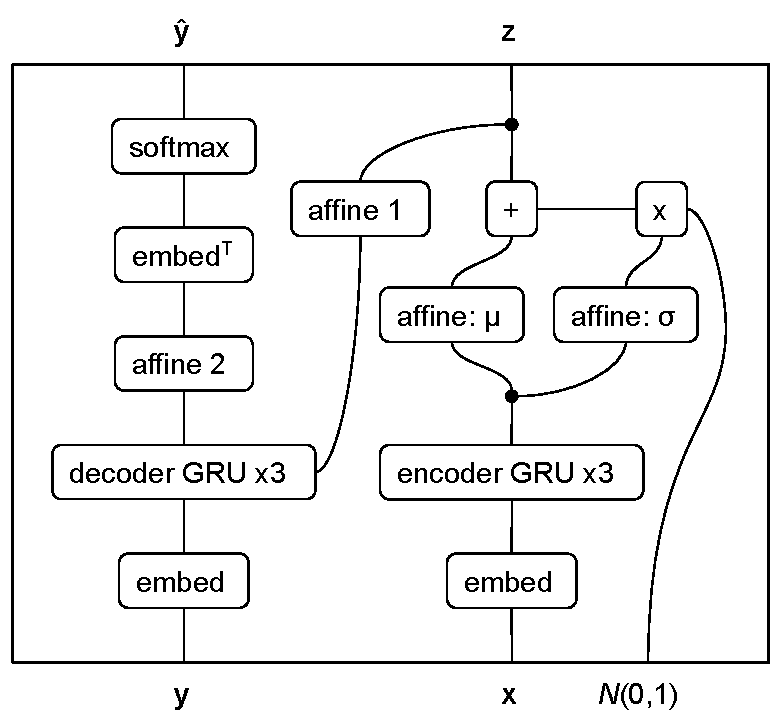
\includegraphics[width=0.7\linewidth]{arch.pdf}
  \caption[]{\label{fig:arch}The architecture.}
\end{figure}

Our model architecture was a recurrent VAE
as described in Section~\ref{sec:recurr-vari-auto} and shown in Figure~\ref{fig:arch}.
The encoder consisted of a linear layer for sentence-piece embedding lookup,
followed by three layers of stacked bidirectional RNNs with gated recurrent units (GRU) \parencite{cho2014learning}.
The final recurrent state was connected to 2 affine layers in parallel
for computing the mean and log variance of the latent variables.
The latent vector was then computed from the mean and variance with random noises during training.
(Outside of training, the latent vector was simply the mean.)
The decoder likewise consisted of a linear layer for sentence-piece embedding lookup,
followed by three layers of unidirectional GRU RNNs
receiving the latent vector after an affine layer as the initial recurrent states.
The recurrent output was connected to an affine layer
followed by a linear layer for predicting the logit probabilities over sentence pieces.
The reconstruction error was softmax cross-entropy.

We applied input-output embedding sharing following \textcite{press2016using}.
Specifically, the two linear input layers for the encoder and the decoder shared the same embedding matrix,
and the linear output layer in the decoder used the transposed matrix.
We found that input-output embedding sharing was only beneficial
when we scaled the weight matrix by \(\sqrt{d}\) for the input layers
with \(d\) being the model dimension.
All weights in the model were initialized according to \textcite{glorot2010understanding}.

The training procedure was stochastic gradient descent with Adam optimization \parencite{kingma2014adam}.
We monitored the reconstruction accuracy on the validation data for hyperparameter tuning.
The optimal model dimension was 512 with the latent dimension doubled due to the bidirectional encoding.
The learning rate was scheduled \(lr / \left( 1 + dr \times \sqrt{s} \right))\) by the training step \(s\),
where \(lr = 0.001\) was the initial learning rate
and \(dr = 0.01\) the decay rate.

We encountered the common problem when using VAEs for language modeling tasks
where the KL loss vanished right at the beginning of training.
This happens when the model simply ignores the encoder and learns the decoder alone to be a language model.
To avoid this problem, we applied KL term weighting and decoder word dropout following \textcite{bowman2015generating}.
The KL weight was scheduled \(\tanh( dr^{2} s )\)
which started from 0 and increased to 1 after \(4e5\) steps.
The word dropout rate was scheduled \(1 / \left( 1 + \exp( dr^{2} s ) \right)\)
which started from 50\% and reduced to 0\% after \(8e5\) steps.

The optimized setting was used for the training of all our models.
We used mini-batches of 100 instances.
For sentence modeling,
we trained the model without sampling for around \(2e5\) steps.
The validation accuracy was over 95\%.
The sentence model did not benefit from sentence-piece sampling due to the large size of the dataset.
We trained a model with sampling for twice as long which still under-performed.
For post modeling,
the model trained without sampling exploded after \(9e5\) steps.
The exact cause was uncertain.
The post model trained with sampling did not converge after almost \(4e6\) steps.
The validation accuracy was still under 60\%.
However, we terminated training since it took 52.5 days and the rate of improvement became increasingly slow.

\subsection{Embedding sentences and posts}\label{sec:embedd-sent-posts}

To embed a sentence or a post using a trained VAE model,
we fed the sequence as input to the encoder and retrieved the latent representation.
We used the model trained without sentence-piece sampling for sentence embedding,
and the model trained with sampling for post embedding.

Since the model trained with sampling could receive the same text with different segmentations
and produce different representations,
we tried a novel approach.
For each text, 128 segmentations were randomly sampled
and the averaged output was taken as the latent representation.
We hypothesized that this averaging method could produce a more robust representation
by factoring away minor variations in the input forms through sampling.

In summary,
we produced a 1024 dimensional embedding for each sentence and post.
For each post, we additionally obtained a sampled embedding.
These embedding vectors were then used for classification and clustering analysis.

\section{Results}\label{sec:results}

\subsection{Classification results}\label{sec:class-results}

We trained logistic classifiers with L2 regularization
to compare against the results reported by \textcite{hasan2014you}
using the same five-fold cross-validation split.

\subsubsection*{Sentence embedding for reason classification}

\begin{table}
  \centering
  \begin{tabular}{lccclccc}
    \toprule
    &\multicolumn{3}{c}{Reason} &&\multicolumn{3}{c}{Stance}\\
    &Baseline &J3 &VAE &&J3 &VAE &VAE-sampled\\
    \midrule
    Abortion  &32.7 &\textbf{39.5} &34.4  &&66.3 &56.75 &56.53\\
    Gay Rights &23.3 &31.4 &\textbf{34.8} &&65.7 &56.10 &55.92\\
    Obama     &19.5 &\textbf{25.1} &20.6  &&69.0 &58.83 &58.73\\
    Marijuana &28.7 &35.1 &\textbf{36.0}  &&64.0 &58.77 &57.65\\
    \bottomrule
  \end{tabular}
  \caption[]{\label{tab:classif}Classification F-scores.}
\end{table}

Table~\ref{tab:classif} shows the reason classification results,
compared against two models Baseline and J3 from \textcite{hasan2014you}.
The Baseline model was a logistic classifier based on ngram, dependency, frame-semantic, quotation, and positional features.
The J3 model used joint density estimation (stance \& reason) with reasons predicted for the preceding post,
which was the best model reported by \textcite{hasan2014you}.
Our logistic classifier (cost = 0.001) using VAE embedding achieved better results on two topics,
but performed worse on the other two.

\subsubsection*{Post embedding for stance classification}

The stance classification results are also included in Table~\ref{tab:classif}.
Our logistic classifier (cost = 0.1) using VAE embedding performed significantly worse than J3,
and did not benefit from the sampled representation.
The post VAE model was under-trained.
Comparing with the sentence VAE,
the main difference was that the posts are much longer than the sentences,
and the recurrent VAE could not reconstruct the sequences well due to the latent bottleneck.

\subsubsection*{Post embedding for topic classification}

We also used the post embedding for topic classification
on the five-fold cross-validation split for the stance dataset,
although \parencite{hasan2014you} did not report results for topic classification.
Our logistic classifier (cost = 0.01) yielded an F-score of 84.6,
using either sampled or unsampled representation.

\subsection{Clustering analysis}\label{sec:clustering-analysis}

We tried to follow the approach of \textcite{boltuvzic2015identifying}
where the sentences were clustered using Hierarchical Agglomerative Clustering (HAC)
and the cluster labels were matched against the reason labels
to compute the Adjusted Rand Score (ARS) and the V-measure (V-MSR).

We trained a L1-regularized logistic classifier to predict the reason label from the sentence embedding.
The regularization would force the classifier to assign non-zero weights to only the dimensions
encoding the most relevant information for differentiating the reasons.
We then removed the irrelevant dimensions from the embedding space and clustered the sentences.
However, the clusters did not match the reason labels.
The ARS and V-MSR were not significantly different from zero.
To investigate further, we turned to analyzing the post embedding.

\subsubsection*{Hierarchical Agglomerative Clustering}

\begin{table}
  \centering
  \begin{tabular}{lccc}
    \toprule
    Cluster & Sampling & ARS & V-MSR \\
    \midrule
    \multirow{2}{*}{Topic} & no & 0.056 &  0.118 \\
    & yes & 0.065 & 0.130 \\[8pt]
    \multirow{2}{*}{Reason} & no & 0.010 &  0.587 \\
    & yes & 0.009 & 0.587 \\[8pt]
    \multirow{2}{*}{Abortion} & no  & 0.014 &  0.551 \\
    & yes & 0.017 & 0.559 \\[8pt]
    \multirow{2}{*}{Gay Rights} & no  & 0.009 &  0.378 \\
    & yes & 0.011 & 0.374 \\
    \multirow{2}{*}{Obama} & no & 0.012 &  0.560 \\
    & yes & 0.013 & 0.555 \\[8pt]
    \multirow{2}{*}{Marijuana} & no  & 0.026 &  0.534 \\
    & yes & 0.037 & 0.535 \\[8pt]
    \bottomrule
  \end{tabular}
  \caption{\label{table:2}Clustering results (ARS and V-MSR) regarding topic, reason, and topic-wise reason.
    Post embedding was used with and without sentence-piece sampling.}
\end{table}

\begin{figure}
  \centering
  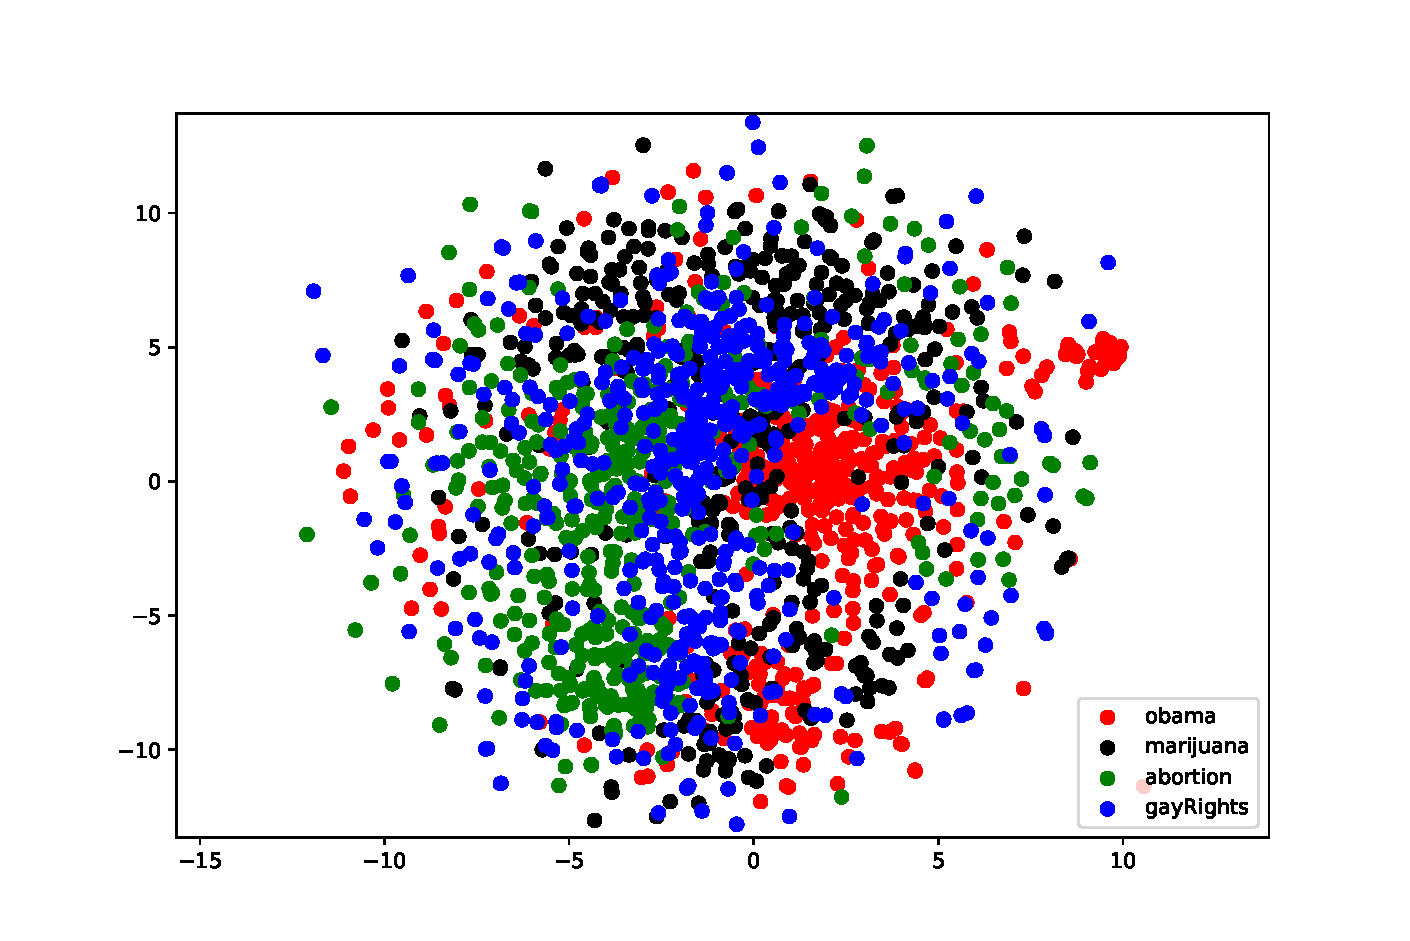
\includegraphics[width=\textwidth]{tsne.pdf}
  \caption{\label{figure:tsne}Post embedding reduced to 2D using t-SNE.}
\end{figure}

We used HAC to cluster the posts and evaluated the clusters against these labels:
the topic, the reason, and the reason within each topic.
The number of clusters was set according to the number of labels.
Table~\ref{table:2} shows the results.
The ARS was consistently low but the scores for the topic label were higher than the rest.
The V-MSR for the topic was low, but significant.
This was consistent with the good topic classification score we found.
Figure~\ref{figure:tsne} visualizes the post embedding space colored by topic
after a dimensionality reduction to 2D using t-SNE \parencite{maaten2008visualizing}.

For all the reason clustering, the V-MSR score was fairly high.
However, this was merely due to the number of clusters being high
as a result of how we assigned the reason labels to posts.
The reason was originally labeled for sentences,
so we took the set of all reasons labeled present in a post as the reason label for that post.
The combination considerably raised the number of labels and consequently the number of clusters.
For example, the number of reason labels for the Obama topic changed form 16 to 101.
As a result, there were many very small clusters and even singleton clusters.
V-MSR was not suited for evaluating such a clustering result.

As the number of reason labels was high and the analysis was further complicated by the fact that the labeling is often quite questionable,
we decided to focus on the stance and topic.

\subsubsection*{Affinity Propagation Clustering}

\begin{table}
  \centering
  \begin{tabular}{lcclccr}
    \toprule
    Dist & Sample & Clusters & Topic & Instances & Cl>50\% & \% \\
    \midrule
    \multirow{8}{*}{euc.} & \multirow{4}{*}{no} & \multirow{4}{*}{49} & Abortion & 463 & 136 & 29.4 \\
         & & & Gay Rights & 560 & 179 & 31.9 \\
         & & & Obama & 446 & 210 & 47.0 \\
         & & & Marijuana & 432 & 104 & 24.1 \\[8pt]
         & \multirow{4}{*}{yes} & \multirow{4}{*}{63} & Abortion & 463 & 107 & 23.1 \\
         & & & Gay Rights & 560 & 165 & 29.5 \\
         & & & Obama & 446 & 210 & 47.1 \\
         & & & Marijuana & 432 & 109 & 25.2\\
    \midrule
    \multirow{8}{*}{cos.} & \multirow{4}{*}{no} & \multirow{4}{*}{198} & Abortion & 463 & 418 & 90.3 \\
         & & & Gay Rights & 560 & 425 & 75.9 \\
         & & & Obama & 446 & 362 & 81.1 \\
         & & & Marijuana & 432 & 386 & 89.4 \\[8pt]
         & \multirow{4}{*}{yes} & \multirow{4}{*}{199} & Abortion & 463 & 428 & \textbf{92.4} \\
         & & & Gay Rights & 560 & 450 & \textbf{80.4} \\
         & & & Obama & 446 & 362 & 81.1 \\
         & & & Marijuana & 432 & 391 & \textbf{90.5} \\
    \bottomrule
  \end{tabular}
  \caption{\label{table:3}APC results for two distance measures (euclidean and cosine)
    and two embedding methods (with and without sentence-piece sampling).
    The number of clusters and instances are listed.
    Additionally, the number and percentage of instances that are in clusters where over 50\% of the instances are of the same topic are shown.}
\end{table}

To further explore the posting embedding, we used Affinity Propagation Clustering (APC).
This clustering method considers all points to be potential exemplars and iteratively groups instances by passing messages between the datapoints until a optimal ordering is achieved \parencite{frey2007clustering}.
Therefore number of clusters is not fixed, but depends on the underlying structure of the data.

APC picked a considerably higher number of clusters compared to what we used for HAC (Table~\ref{table:3}).
We tried two distance measures, euclidean and cosine.
The results were very different.
When using cosine, the number of clusters was 4--5 times higher.
To explore how the clusters represented different topics,
we analyzed for each topic how many of its instances were in clusters where they were the majority (>50\%).
Here, cosine provided much better results.
This is understandable considering that the euclidean metric often does not work well in high dimensional spaces.
The results also suggest that the embedding produced with sentence-piece sampling yielded better clusters.
% For all topics, over 80\% of its instances were placed in clusters where this topic formed a majority.
% Our explorations suggest that the posts were ordered in a meaningful way in the embedding space by the VAE regarding their topics.
% But ordering does not correspond to a simple 4 topics = 4 clusters formula.
% A sequence of text is rich in information on many levels (like semantic, syntactic, etc.).
% This results in a more nuanced embedding space, for which in order to fully comprehend its structure, further research is needed.

\section{Conclusion}\label{sec:conclusion}

VAEs are simple generative models for learning argumentation representation requiring only raw texts for training.
The encoder could be used to embed texts for further discriminative modeling.
Our sentence model performed relatively well on reason classification
despite the disparity between the cleanliness of the training data and the messiness of the evaluation data.
However, the same embedded representation did not work well when used for clustering.

Training a VAE on long sequences such as whole posts was difficult.
Our under-trained post model did not produce adequate representation for stance classification.
Further analysis via clustering showed that the learned latent space
was locally arranged to some extent according to the topic of discussion.
However, globally, the latent space was not simply separable by the topic or the reason of argumentation.

We attempted at charting the latent space by manually introspecting the clusters,
which turned out to be extremely difficult.
The clusters were not formed according to easily recognizable patterns.
We did discover that some clusters contained posts in the same thread
due to literal quoting of previous posts in a chain of discussion.
Interestingly, within almost all the clusters,
the shortest posts were the closest to the centroid.
We tried generating posts from the centroids using the decoder with greedy decoding,
but the generated texts were mostly lengthy ramblings with no coherent content.

Nevertheless we are optimistic about the research potential along this approach.
The training method could be adjusted to incorporate the desired argumentation labeling.
Take our sentence VAE for example,
the reconstruction accuracy exceeded 95\%,
but for the purpose of argumentation mining,
we are not as interested in the exact wording or the syntactic structure
as we are in the semantic and pragmatic aspects.
The VAE model could be trained with paraphrasing datasets
to regularize the latent space for the desired abstraction.
Apart from the usage of embedding,
a well-trained VAE has unparalleled prospects for argumentation generation
due to the disentanglement of features in the latent representation.

\printbibliography[]

\end{document}
